%%% PREAMBLE - Do not touch %%%%%%%%%%%%%%%%%%%%%%%%%%%%%%%%%%%%%%%%%%%%%%%%%%%%%%
\documentclass[10pt,twocolumn,letterpaper]{article}
\usepackage[ansinew]{inputenc}
\usepackage[portuges,brazil,english]{babel}
\usepackage{model}
\usepackage{times}
\usepackage{epsfig}
\usepackage{graphicx}
\usepackage{amsmath}
\usepackage{amssymb}
\usepackage{color}
\usepackage[pagebackref=true,breaklinks=true,letterpaper=true,colorlinks,bookmarks=false]{hyperref}
%  ABACO -- Conjunto de macros para desenhar o 'abaco
%  Desenho original de Hans Liesenberg
%  Macros de Tomasz Kowaltowski
%  DCC -- IMECC -- UNICAMP
%  Mar,co de 1988  --  Vers~ao 1.0
% Ajustado para LaTeX da SUN -- Mar,co de 1991
% ---------------------------------------------------------
%  Chamada:   \ABACO{d1}{d2}{d3}{d4}{esc}
%             com:  di's -- os quatro d'igitos;
%                   esc  -- fator de escala
% ---------------------------------------------------------
%  DEFINI,C~OES AUXILIARES
% ---------------------------------------------------------
%  Forma o d'igito pequeno (0 ou 1)

\newcommand{\ABACODP}[1]{%
%
\thicklines
%    
\begin{picture}(8,0)
    \ifcase#1{   %  caso 0
       \put(0,0)    {\line(1,0){4}}
       \multiput(5,0)(2,0){2}{\oval(2,4)}}
    \or{         %  caso 1
       \put(2,0)    {\line(1,0){4}}
       \multiput(1,0)(6,0){2}{\oval(2,4)}}
    \fi
\end{picture}
    } % \ABACODP

% Forma o d'igito grande (0 a 4)

\newcommand{\ABACODG}[1]{%
%
\thicklines
%    
\begin{picture}(14,0)
    \ifcase#1{   % caso 0
       \multiput(1,0)(2,0){5}{\oval(2,4)}}
       \put(10,0)   {\line(1,0){4}}
    \or{         % caso 1
       \multiput(1,0)(2,0){4}{\oval(2,4)}}
       \put(8,0)   {\line(1,0){4}}
       \put(13,0)   {\oval(2,4)}
    \or{         % caso 2
       \multiput(1,0)(2,0){3}{\oval(2,4)}
       \put(6,0)   {\line(1,0){4}}
       \multiput(11,0)(2,0){2}{\oval(2,4)}}
    \or{         % caso 3
       \multiput(1,0)(2,0){2}{\oval(2,4)}
       \put(4,0)   {\line(1,0){4}}
       \multiput(9,0)(2,0){3}{\oval(2,4)}}
    \or{         % caso 4
       \put(1,0)  {\oval(2,4)}}
       \put(2,0)   {\line(1,0){4}}
       \multiput(7,0)(2,0){4}{\oval(2,4)}
    \fi
\end{picture}
    } % \ABACODG
       
% Forma um d'igito (0 a 9)

\newcommand{\ABACOD}[1]{%
%
    \ifnum#1>9
       \errmessage{#1: Argumento invalido para ABACO}
    \fi
    \ifnum#1<0
       \errmessage{#1: Argumento invalido para ABACO}
    \fi
%
\begin{picture}(24,0)
%    
    \ifnum#1<5
       \put(16,0) {\ABACODP{0}}
    \else   
       \put(16,0) {\ABACODP{1}}
    \fi
%    
    \ifnum#1<5
       \put(0,0)  {\ABACODG{#1}}
    \else
       \ifcase#1\or \or \or \or
          \or  \put(0,0)  {\ABACODG{0}}
          \or  \put(0,0)  {\ABACODG{1}}
          \or  \put(0,0)  {\ABACODG{2}}
          \or  \put(0,0)  {\ABACODG{3}}
          \or  \put(0,0)  {\ABACODG{4}}
       \fi
    \fi   
\end{picture}
    } % \ABACOD
    
% -------------------------------------------------

%  DEFINI,C~AO PRINCIPAL
    
\newcommand{\ABACO}[5]{%
    \setlength{\unitlength}{#5mm}
%
    \thinlines
%   
\begin{picture}(28,25)
%   
% moldura
%
% externa
%
        \put(0,0)            {\line(0,1){25}}
        \put(0,0)            {\line(1,0){28}}
        \put(28,0)           {\line(0,1){25}}
        \put(0,25)           {\line(1,0){28}}
% interna
        \put(2,2)            {\line(0,1){21}}
        \put(26,2)           {\line(0,1){21}}
        \put(16,2)           {\line(0,1){21}}
        \put(18,2)           {\line(0,1){21}}
        \put(2,2)            {\line(1,0){14}}
%        \put(16,2)           {\line(1,-1){1}}
%        \put(17,1)           {\line(1,1){1}}
        \put(18,2)           {\line(1,0){8}}
        \put(2,23)           {\line(1,0){14}}
%        \put(16,23)          {\line(1,1){1}}
%       \put(17,24)          {\line(1,-1){1}}
        \put(18,23)          {\line(1,0){8}}
%        \put(0,0)            {\line(1,1){2}}
%        \put(0,25)           {\line(1,-1){2}}
%        \put(28,0)           {\line(-1,1){2}}
%        \put(28,25)          {\line(-1,-1){2}}
%
%   
% d'igitos
%
%   
       \put(2,20)  {\ABACOD{#1}}
       \put(2,15)  {\ABACOD{#2}}
       \put(2,10)  {\ABACOD{#3}}
       \put(2,5)   {\ABACOD{#4}}
%      
\end{picture}
    } % \ABACO
    


\cvprfinalcopy % *** Uncomment this line for the final submission
\def\httilde{\mbox{\tt\raisebox{-.5ex}{\symbol{126}}}}
\ifcvprfinal\pagestyle{empty}\fi

\newcommand{\TODO}[1]{TODO: #1}
\newcommand{\CITEONE}[2]{\mbox{#1 \cite{#2}}}
\newcommand{\CITETWO}[3]{\mbox{#1 and #2 \cite{#3}}}
\newcommand{\CITEN}[2]{\mbox{#1 et al. \cite{#2}}}

%%% Report beginning %%%%%%%%%%%%%%%%%%%%%%%%%%%%%%%%%%%%%%%%%%%%%%%%%%%%%%%%%%%%%%
\begin{document}

%%% Title and authors %%%%%%%%%%%%%%%%%%%%%%%%%%%%%%%%%%%%%%%%%%%%%%%%%%%%%%%%%%%%
\title{MC886 - Assignment 1\\
Predicting social network shares using Linear Regression}
\author{Gustavo de Mello Crivelli\thanks{Undergrad student in the Institute of Computing, University of Campinas (Unicamp). \textbf{Contact}: \tt\small{gmcrivelli@gmail.com}}\\
RA 136008}

%%% Abstract %%%%%%%%%%%%%%%%%%%%%%%%%%%%%%%%%%%%%%%%%%%%%%%%%%%%%%%%%%%%%%%%%%%%%
\maketitle
\begin{abstract}
Using a dataset of over 30.000 \CITEONE{entries}{Dataset}, Python was used to build and train a predictor for the number of times a given publication will be shared in social networks. A separate dataset was then used for testing. An initial attempt with only basic linear regression was able to make predictions with an error of 3183 shares, and managed to predict 2.6\% of the test dataset with an error of 100 shares. Further optimizations using Gradient Descent, feature scaling and regularization led to a final predictor able to guess shares with an error of 2788 shares, and had 8.3\% of predictions within 100 shares of the correct value.
\end{abstract}

%%% Introduction %%%%%%%%%%%%%%%%%%%%%%%%%%%%%%%%%%%%%%%%%%%%%%%%%%%%%%%%%%%%%%%%%
\section{Introduction}

Social networks are bustling hubs of information exchange. Being able to predict how far an article might go in terms of social network sharing, as well as understanding what makes a publication become viral, is invaluable for any content creator.

This report details the process of attempting to build a predictor able to do the above, using a range of Linear Regression and Gradient Descent techniques.

\subsection{Dataset}

The dataset used for this work was published by \hyperlink{www.mashable.com}{www.mashable.com}\CITEONE{}{Dataset}. Their content as the rights to reproduce it belongs to them. Hence, this dataset does not share the original content but some statistics associated with it\CITEONE{}{Portugal}.

The training dataset contains 31715 entries, each with 58 total predictive attributes and a target attribute (the number of shares). Each feature has a different value range, and some of them are discrete. All of this needs to be dealt with in order to achieve better results in prediction.

The test dataset contains 7929 entries and is similar to the training dataset in terms of attributes. It is used to validate the predictor learned while using the training dataset.

%%% Add section %%%%%%%%%%%%%%%%%%%%%%%%%%%%%%%%%%%%%%%%%%%%%%%%%%%%%%%%%%%%%%%%%%
\section{Proposed Solutions}
All results are listed in the Results and Discussion section.

\subsection{Linear Regression}

The first attempt was made using basic linear regression. Given a dataset $X$ with $m$ entries, an entry $x^{(i)}$ from that dataset and a target value $y^{(i)}$, we want to find an array of coefficients $\theta$ such that, given $h_\theta(x) = \theta \cdot x$, the cost function $J(\theta) = \frac{1}{2m}\sum_{i=1}^{m}(h_\theta(x^{(i)}) - y^{(i)})^2$ is \CITEONE{minimal}{Classroom}. 

For this, \CITEONE{scikit-learn}{scikit-learn} was used. No further optimizations were done at this time.

\subsection{Feature Scaling}

The second proposed solution utilized the same linear regression as above, but normalized the features in the training to keep their values in the range $[0,1]$. The test dataset was also normalized, using the same parameters found during the training set normalization. 

Surprisingly, this performed with worse results than the non-normalized attempt.

\subsection{Gradient Descent}
\label{sec:gd}

The third proposed solution moved on to Gradient Descent. Let $n$ be the number of coefficients in the $\theta$ array. In order to find the minimum cost of $J(\theta)$, the coefficient array $\theta$ is iteratively updated until the function converges. This is described by $\theta_j := \theta_j - \alpha\frac{\delta}{\delta\theta_j}J(\theta)$ for $0 \leq j < n$, where $\alpha$ is a scalar representing the learning rate.

The feature scaling proposed above was also used in this and in the following proposed solutions. For this solution, 10000 iterations were made, and an initial $\theta$ was built with random values in the range $(-1000,1000)$. 

Figure \ref{fig:gd1} details the variations in the mean absolute error of predicted shares as the training iterates. The high values are a good indication of overfitting to the training dataset, and this will need to be dealt with.

\begin{figure}
\begin{center}
	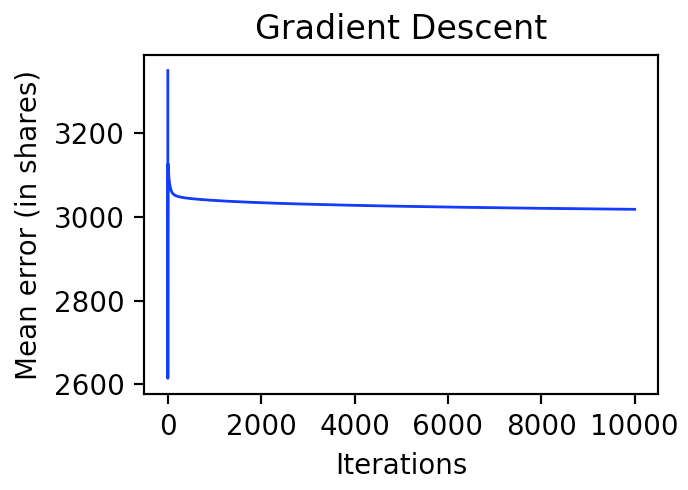
\includegraphics[width=0.99\columnwidth]{pics/gd1.png}
	\caption{Mean error by Gradient Descent iteration.\label{fig:gd1}}   
\end{center} 
\end{figure} 

\subsection{Gradient Descent with Feature Dropping}
\label{sec:gdfd}

The next step was to remove superfluous features that might be contributing with noise, and leading the predictor to overfit to the training data. For this, the coefficient array found in the previous round of training was analyzed, and every feature whose corresponding coefficient had an absolute value inferior to 1000 was removed from consideration.

After this procedure, the only features still in consideration were the ones in the set $F = {6,8,11,18,22,23,24,25,26,27,28,29,30,29,41,43}$. (Please reference the \CITEONE{dataset}{Dataset} for more details.

Furthermore, the dataset itself was filtered, and entries with anomalous features were removed. For instance, all entries marked as having zero words in the content (Feature 3), were likely the result of a malformed observation, as can be easily verified by accessing the link to the publication in that entry.

The results of these changes can be seen in Figure \ref{fig:gd2}

\begin{figure}
\begin{center}
	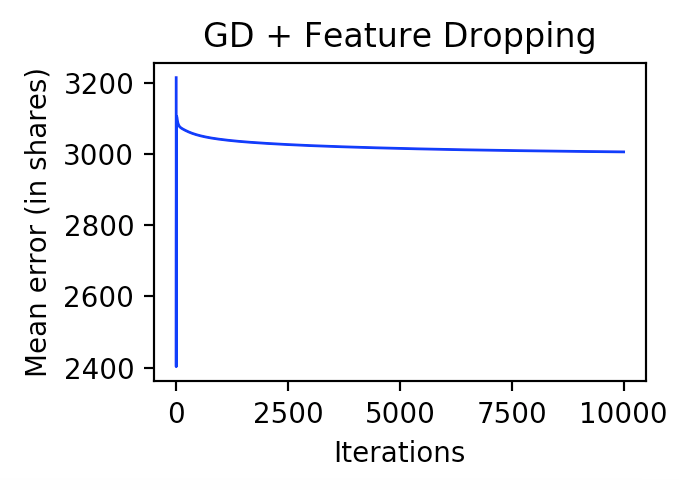
\includegraphics[width=0.99\columnwidth]{pics/gd2.png}
	\caption{Mean error by Gradient Descent iteration, with feature dropping.\label{fig:gd2}}   
\end{center} 
\end{figure}

\subsection{Gradient Descent with Regularization}
\label{sec:gdr}

It was then attempted to build a more complex predictor by changing $h_\theta(x)$ to be a second-degree polynomial function. For this, a new feature array was produced for each entry, composed of an array of the features mentioned in the previous step, concatenated with an array containing the square of those features.

To minimize overfitting, a $\lambda$ regularization parameter was introduced, so that the cost function becomes $J(\theta) = \frac{1}{2m}(\sum_{i=1}^{m}(h_\theta(x^{(i)}) - y^{(i)})^2 + \lambda\sum_{j=1}^{n}\theta_{j}^{2})$. The intent of this is to penalize more complex models over simpler ones, in a way that will reinforce important features while reducing the influence of noise.

The lambda with the best results was found to be $\lambda = 1000$. The results of these changes can be seen in Figure \ref{fig:gd3}

\begin{figure}
\begin{center}
	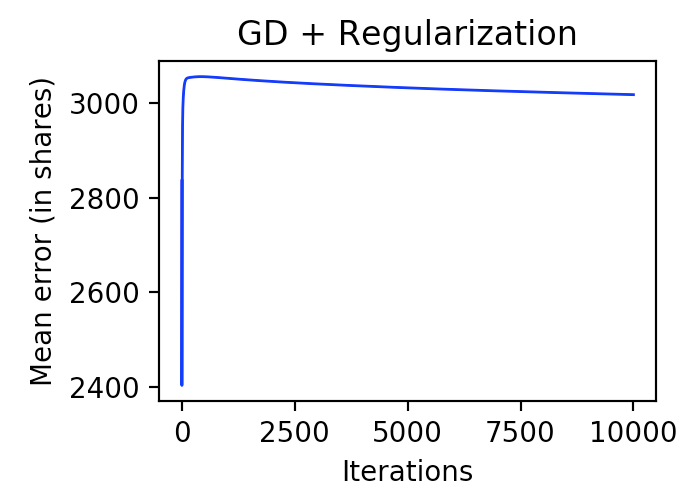
\includegraphics[width=0.99\columnwidth]{pics/gd3.png}
	\caption{Mean error by Gradient Descent iteration, with feature dropping and regularization.\label{fig:gd3}}   
\end{center} 
\end{figure}

\subsection{Gradient Descent with Further Feature Dropping}
\label{sec:gdrfd}

A second attempt was made at choosing the most relevant features. Instead of only taking the features with the highest coefficients, the following algorithm was executed:

\begin{enumerate}
    \item Start with an empty set of selected features $F$.
    \item For every feature $f$ in the dataset that is still not in $F$, train and evaluate the predictor using only $F \cup \{f, f^2\}$ as features.
    \item Select the feature $f$ that resulted in the lowest mean error in Step 2. If it is lower than the previous mean error, add $\{f, f^2\}$ permanently to $F$. Otherwise, stop.
    \item Repeat from Step 2.
\end{enumerate}

Using this, a new set of features was selected, composed of features $F = {6,7,8,19,21,25,27,29,35}$. This takes care of the discrete features, as the only remaining discrete feature is Feature 25 (whether or not the article was published on a Friday). The results of this filtering can be seen in Figure \ref{fig:gd4}, and are considerably better than in the previous attempts.

\begin{figure}
\begin{center}
	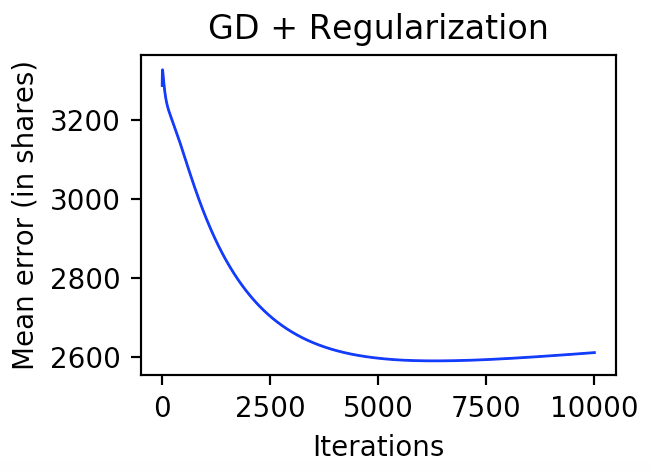
\includegraphics[width=0.99\columnwidth]{pics/gd4.png}
	\caption{Mean error by Gradient Descent iteration, with further feature dropping and regularization.\label{fig:gd4}} 
\end{center} 
\end{figure}

\subsection{Normal Equations}

At this point, a different direction was attempted by using Normal Equations to analytically solve the regression. All of the techniques adopted regarding dataset filtering and feature processing were also applied here. 

Since calculating $\theta$ in this manner requires a lot of computing power, a smaller sample of the original dataset was used. This contained the first $10000$ entries that were considered to be usable.

%%% Add section %%%%%%%%%%%%%%%%%%%%%%%%%%%%%%%%%%%%%%%%%%%%%%%%%%%%%%%%%%%%%%%%%%
\section{Results and Discussion}

Table \ref{table:results} contains the results of the above experimentation.

\begin{table*}
\begin{center}
    \begin{tabular}{ | l | l | l | l |}
    \hline
     & \textbf{Mean error} & \textbf{Accuracy within 500 shares} & \textbf{Accuracy within 100 shares} \\ \hline
    \textbf{(2.1)} Linear Regression (LR) & 3183.5 & 14.6\% & 2.6\% \\ \hline
    \textbf{(2.2)} LR + Feature Scaling & 3306.2 & 13.8\% & 2.7\% \\ \hline
    \textbf{(2.3)} Gradient Descent (GD) & 3194.3 & 11.5\% & 2.2\% \\ \hline
    \textbf{(2.4)} GD + Feature Dropping (FD) & 3199.4 & 9.9\% & 2.0\% \\ \hline
    \textbf{(2.5)} GD + FD + Regularization (Reg) & 3228.2 & 9.7\% & 1.9\% \\ \hline
    \textbf{(2.6)} GD + Reg + Further FD & 2789.5 & 33.3\% & 8.3\% \\ \hline
    \textbf{(2.7)} Normal Equations & 3176.5 & 17.7\% & 3.2\% \\ 
    \hline
    \end{tabular}
    \caption{Comparison of the results obtained.\label{table:results}} 
\end{center}  
\end{table*}

Surprisingly, every technique implemented seemed to deliver progressively worse results. This may have been because of the amount of noise contained in the dataset, as is suggested by the drastic improvement in the results once the features were re-analyzed and re-selected.

The results obtained when Normal Equations were attempted indicate that it is able to reach the same results as the Gradient Descent method. However, due to its increased demand of memory and computing power, such a method is only feasible by either selecting a smaller subset of training examples, or by some other manner of training in batches that may allow the usage of all training examples (although this was not done here).

As for the learning rates applied in Gradient Descent implementations, it was found through experimentation that for implementations \hyperref[sec:gd]{2.3}, \hyperref[sec:gdfd]{2.4} and \hyperref[sec:gdr]{2.5}, the optimal learning rate was $\alpha = 0.1$, as larger values caused the training to diverge and smaller values were simply slower to converge. For implementation \hyperref[sec:gdrfd]{2.6}, the optimal learning rate was found to be $\alpha = 0.05$.

%%% Add section %%%%%%%%%%%%%%%%%%%%%%%%%%%%%%%%%%%%%%%%%%%%%%%%%%%%%%%%%%%%%%%%%%
\section{Conclusions and Future Work}
Linear regression and Gradient Descent are the most basic of Machine Learning tools. However, it is possible to increment those with more advanced techniques in order to achieve better results, as was shown by the results obtained by experimentation. 

That it was possible to predict shares with a mean absolute error of 2789.5 leads to a few conclusions. First, predicting social network shares is absolutely possible, as the predictor did get better at it as more techniques were implemented. 

Second, it may be that the current model is not complex enough to properly predict shares, and more advanced techniques such as Deep Learning are likely to deliver better results. 

Finally, if you are going to publish something, it is probably a good idea to do it on a Friday.
%%% References %%%%%%%%%%%%%%%%%%%%%%%%%%%%%%%%%%%%%%%%%%%%%%%%%%%%%%%%%%%%%%%%%%%
{\small
\bibliographystyle{unsrt}
\bibliography{refs}
}

\end{document}